\documentclass[1p]{elsarticle_modified}
%\bibliographystyle{elsarticle-num}

%\usepackage[colorlinks]{hyperref}
%\usepackage{abbrmath_seonhwa} %\Abb, \Ascr, \Acal ,\Abf, \Afrak
\usepackage{amsfonts}
\usepackage{amssymb}
\usepackage{amsmath}
\usepackage{amsthm}
\usepackage{scalefnt}
\usepackage{amsbsy}
\usepackage{kotex}
\usepackage{caption}
\usepackage{subfig}
\usepackage{color}
\usepackage{graphicx}
\usepackage{xcolor} %% white, black, red, green, blue, cyan, magenta, yellow
\usepackage{float}
\usepackage{setspace}
\usepackage{hyperref}

\usepackage{tikz}
\usetikzlibrary{arrows}

\usepackage{multirow}
\usepackage{array} % fixed length table
\usepackage{hhline}

%%%%%%%%%%%%%%%%%%%%%
\makeatletter
\renewcommand*\env@matrix[1][\arraystretch]{%
	\edef\arraystretch{#1}%
	\hskip -\arraycolsep
	\let\@ifnextchar\new@ifnextchar
	\array{*\c@MaxMatrixCols c}}
\makeatother %https://tex.stackexchange.com/questions/14071/how-can-i-increase-the-line-spacing-in-a-matrix
%%%%%%%%%%%%%%%

\usepackage[normalem]{ulem}

\newcommand{\msout}[1]{\ifmmode\text{\sout{\ensuremath{#1}}}\else\sout{#1}\fi}
%SOURCE: \msout is \stkout macro in https://tex.stackexchange.com/questions/20609/strikeout-in-math-mode

\newcommand{\cancel}[1]{
	\ifmmode
	{\color{red}\msout{#1}}
	\else
	{\color{red}\sout{#1}}
	\fi
}

\newcommand{\add}[1]{
	{\color{blue}\uwave{#1}}
}

\newcommand{\replace}[2]{
	\ifmmode
	{\color{red}\msout{#1}}{\color{blue}\uwave{#2}}
	\else
	{\color{red}\sout{#1}}{\color{blue}\uwave{#2}}
	\fi
}

\newcommand{\Sol}{\mathcal{S}} %segment
\newcommand{\D}{D} %diagram
\newcommand{\A}{\mathcal{A}} %arc


%%%%%%%%%%%%%%%%%%%%%%%%%%%%%5 test

\def\sl{\operatorname{\textup{SL}}(2,\Cbb)}
\def\psl{\operatorname{\textup{PSL}}(2,\Cbb)}
\def\quan{\mkern 1mu \triangleright \mkern 1mu}

\theoremstyle{definition}
\newtheorem{thm}{Theorem}[section]
\newtheorem{prop}[thm]{Proposition}
\newtheorem{lem}[thm]{Lemma}
\newtheorem{ques}[thm]{Question}
\newtheorem{cor}[thm]{Corollary}
\newtheorem{defn}[thm]{Definition}
\newtheorem{exam}[thm]{Example}
\newtheorem{rmk}[thm]{Remark}
\newtheorem{alg}[thm]{Algorithm}

\newcommand{\I}{\sqrt{-1}}
\begin{document}

%\begin{frontmatter}
%
%\title{Boundary parabolic representations of knots up to 8 crossings}
%
%%% Group authors per affiliation:
%\author{Yunhi Cho} 
%\address{Department of Mathematics, University of Seoul, Seoul, Korea}
%\ead{yhcho@uos.ac.kr}
%
%
%\author{Seonhwa Kim} %\fnref{s_kim}}
%\address{Center for Geometry and Physics, Institute for Basic Science, Pohang, 37673, Korea}
%\ead{ryeona17@ibs.re.kr}
%
%\author{Hyuk Kim}
%\address{Department of Mathematical Sciences, Seoul National University, Seoul 08826, Korea}
%\ead{hyukkim@snu.ac.kr}
%
%\author{Seokbeom Yoon}
%\address{Department of Mathematical Sciences, Seoul National University, Seoul, 08826,  Korea}
%\ead{sbyoon15@snu.ac.kr}
%
%\begin{abstract}
%We find all boundary parabolic representation of knots up to 8 crossings.
%
%\end{abstract}
%\begin{keyword}
%    \MSC[2010] 57M25 
%\end{keyword}
%
%\end{frontmatter}

%\linenumbers
%\tableofcontents
%
\newcommand\colored[1]{\textcolor{white}{\rule[-0.35ex]{0.8em}{1.4ex}}\kern-0.8em\color{red} #1}%
%\newcommand\colored[1]{\textcolor{white}{ #1}\kern-2.17ex	\textcolor{white}{ #1}\kern-1.81ex	\textcolor{white}{ #1}\kern-2.15ex\color{red}#1	}

{\Large $\underline{12a_{0671}~(K12a_{0671})}$}

\setlength{\tabcolsep}{10pt}
\renewcommand{\arraystretch}{1.6}
\vspace{1cm}\begin{tabular}{m{100pt}>{\centering\arraybackslash}m{274pt}}
\multirow{5}{120pt}{
	\centering
	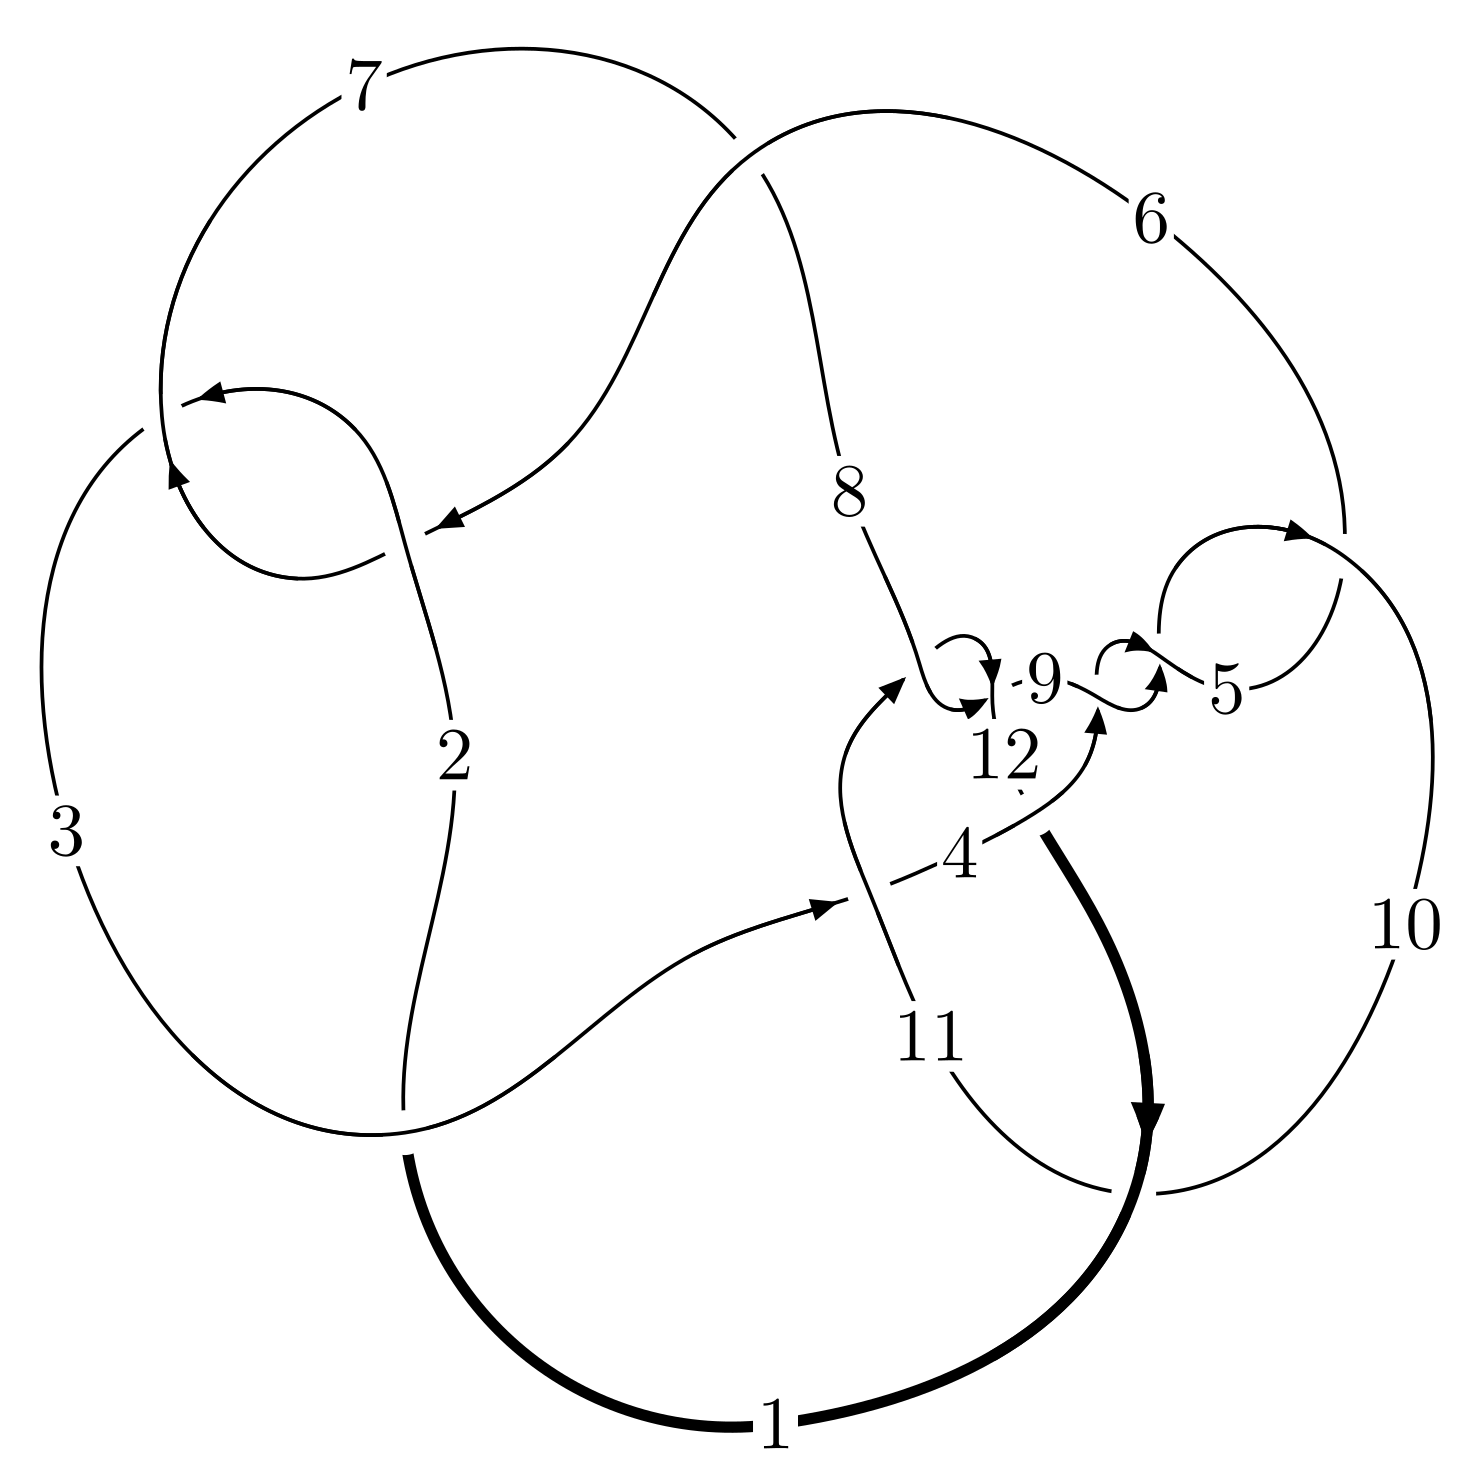
\includegraphics[width=112pt]{../../../GIT/diagram.site/Diagrams/png/1472_12a_0671.png}\\
\ \ \ A knot diagram\footnotemark}&
\allowdisplaybreaks
\textbf{Linearized knot diagam} \\
\cline{2-2}
 &
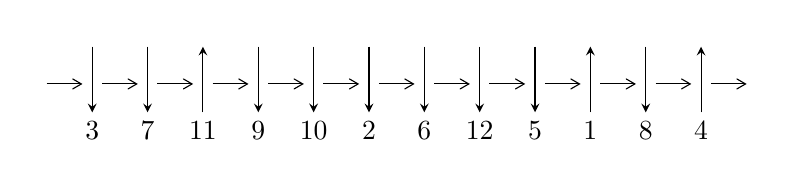
\begin{tikzpicture}[x=20pt, y=17pt]
	% nodes
	\node (C0) at (0, 0) {};
	\node (C1) at (1, 0) {};
	\node (C1U) at (1, +1) {};
	\node (C1D) at (1, -1) {3};

	\node (C2) at (2, 0) {};
	\node (C2U) at (2, +1) {};
	\node (C2D) at (2, -1) {7};

	\node (C3) at (3, 0) {};
	\node (C3U) at (3, +1) {};
	\node (C3D) at (3, -1) {11};

	\node (C4) at (4, 0) {};
	\node (C4U) at (4, +1) {};
	\node (C4D) at (4, -1) {9};

	\node (C5) at (5, 0) {};
	\node (C5U) at (5, +1) {};
	\node (C5D) at (5, -1) {10};

	\node (C6) at (6, 0) {};
	\node (C6U) at (6, +1) {};
	\node (C6D) at (6, -1) {2};

	\node (C7) at (7, 0) {};
	\node (C7U) at (7, +1) {};
	\node (C7D) at (7, -1) {6};

	\node (C8) at (8, 0) {};
	\node (C8U) at (8, +1) {};
	\node (C8D) at (8, -1) {12};

	\node (C9) at (9, 0) {};
	\node (C9U) at (9, +1) {};
	\node (C9D) at (9, -1) {5};

	\node (C10) at (10, 0) {};
	\node (C10U) at (10, +1) {};
	\node (C10D) at (10, -1) {1};

	\node (C11) at (11, 0) {};
	\node (C11U) at (11, +1) {};
	\node (C11D) at (11, -1) {8};

	\node (C12) at (12, 0) {};
	\node (C12U) at (12, +1) {};
	\node (C12D) at (12, -1) {4};
	\node (C13) at (13, 0) {};

	% arrows
	\draw[->,>={angle 60}]
	(C0) edge (C1) (C1) edge (C2) (C2) edge (C3) (C3) edge (C4) (C4) edge (C5) (C5) edge (C6) (C6) edge (C7) (C7) edge (C8) (C8) edge (C9) (C9) edge (C10) (C10) edge (C11) (C11) edge (C12) (C12) edge (C13) ;	\draw[->,>=stealth]
	(C1U) edge (C1D) (C2U) edge (C2D) (C3D) edge (C3U) (C4U) edge (C4D) (C5U) edge (C5D) (C6U) edge (C6D) (C7U) edge (C7D) (C8U) edge (C8D) (C9U) edge (C9D) (C10D) edge (C10U) (C11U) edge (C11D) (C12D) edge (C12U) ;
	\end{tikzpicture} \\
\hhline{~~} \\& 
\textbf{Solving Sequence} \\ \cline{2-2} 
 &
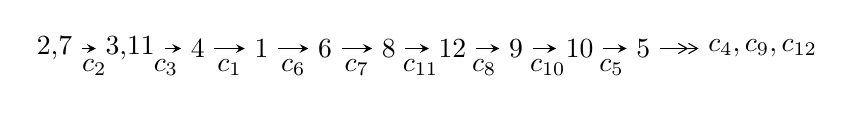
\begin{tikzpicture}[x=23pt, y=7pt]
	% node
	\node (A0) at (-1/8, 0) {2,7};
	\node (A1) at (17/16, 0) {3,11};
	\node (A2) at (17/8, 0) {4};
	\node (A3) at (25/8, 0) {1};
	\node (A4) at (33/8, 0) {6};
	\node (A5) at (41/8, 0) {8};
	\node (A6) at (49/8, 0) {12};
	\node (A7) at (57/8, 0) {9};
	\node (A8) at (65/8, 0) {10};
	\node (A9) at (73/8, 0) {5};
	\node (C1) at (1/2, -1) {$c_{2}$};
	\node (C2) at (13/8, -1) {$c_{3}$};
	\node (C3) at (21/8, -1) {$c_{1}$};
	\node (C4) at (29/8, -1) {$c_{6}$};
	\node (C5) at (37/8, -1) {$c_{7}$};
	\node (C6) at (45/8, -1) {$c_{11}$};
	\node (C7) at (53/8, -1) {$c_{8}$};
	\node (C8) at (61/8, -1) {$c_{10}$};
	\node (C9) at (69/8, -1) {$c_{5}$};
	\node (A10) at (11, 0) {$c_{4},c_{9},c_{12}$};

	% edge
	\draw[->,>=stealth]	
	(A0) edge (A1) (A1) edge (A2) (A2) edge (A3) (A3) edge (A4) (A4) edge (A5) (A5) edge (A6) (A6) edge (A7) (A7) edge (A8) (A8) edge (A9) ;
	\draw[->>,>={angle 60}]	
	(A9) edge (A10);
\end{tikzpicture} \\ 

\end{tabular} \\

\footnotetext{
The image of knot diagram is generated by the software ``\textbf{Draw programme}" developed by Andrew Bartholomew(\url{http://www.layer8.co.uk/maths/draw/index.htm\#Running-draw}), where we modified some parts for our purpose(\url{https://github.com/CATsTAILs/LinksPainter}).
}\phantom \\ \newline 
\centering \textbf{Ideals for irreducible components\footnotemark of $X_{\text{par}}$} 
 
\begin{align*}
I^u_{1}&=\langle 
-1.92237\times10^{100} u^{108}-3.61566\times10^{100} u^{107}+\cdots+1.78606\times10^{100} b-3.08465\times10^{100},\\
\phantom{I^u_{1}}&\phantom{= \langle  }-2.89446\times10^{101} u^{108}-5.42772\times10^{101} u^{107}+\cdots+1.78606\times10^{100} a-1.31985\times10^{101},\\
\phantom{I^u_{1}}&\phantom{= \langle  }u^{109}+u^{108}+\cdots+10 u-1\rangle \\
I^u_{2}&=\langle 
- u^{20}- u^{19}+\cdots+b-3,\;- u^{22}+2 u^{21}+\cdots+a-1,\;u^{23}-5 u^{21}+\cdots-3 u+1\rangle \\
\\
\end{align*}
\raggedright * 2 irreducible components of $\dim_{\mathbb{C}}=0$, with total 132 representations.\\
\footnotetext{All coefficients of polynomials are rational numbers. But the coefficients are sometimes approximated in decimal forms when there is not enough margin.}
\newpage
\renewcommand{\arraystretch}{1}
\centering \section*{I. $I^u_{1}= \langle -1.92\times10^{100} u^{108}-3.62\times10^{100} u^{107}+\cdots+1.79\times10^{100} b-3.08\times10^{100},\;-2.89\times10^{101} u^{108}-5.43\times10^{101} u^{107}+\cdots+1.79\times10^{100} a-1.32\times10^{101},\;u^{109}+u^{108}+\cdots+10 u-1 \rangle$}
\flushleft \textbf{(i) Arc colorings}\\
\begin{tabular}{m{7pt} m{180pt} m{7pt} m{180pt} }
\flushright $a_{2}=$&$\begin{pmatrix}1\\0\end{pmatrix}$ \\
\flushright $a_{7}=$&$\begin{pmatrix}0\\u\end{pmatrix}$ \\
\flushright $a_{3}=$&$\begin{pmatrix}1\\u^2\end{pmatrix}$ \\
\flushright $a_{11}=$&$\begin{pmatrix}16.2058 u^{108}+30.3893 u^{107}+\cdots-103.585 u+7.38970\\1.07632 u^{108}+2.02437 u^{107}+\cdots-24.4693 u+1.72707\end{pmatrix}$ \\
\flushright $a_{4}=$&$\begin{pmatrix}16.1376 u^{108}+29.6267 u^{107}+\cdots-211.100 u+13.6064\\-0.507290 u^{108}+0.244275 u^{107}+\cdots-19.1382 u+2.40150\end{pmatrix}$ \\
\flushright $a_{1}=$&$\begin{pmatrix}- u^2+1\\- u^4\end{pmatrix}$ \\
\flushright $a_{6}=$&$\begin{pmatrix}u\\u\end{pmatrix}$ \\
\flushright $a_{8}=$&$\begin{pmatrix}- u^3\\- u^3+u\end{pmatrix}$ \\
\flushright $a_{12}=$&$\begin{pmatrix}13.4025 u^{108}+25.0901 u^{107}+\cdots-70.9837 u+3.69015\\2.66737 u^{108}+4.81907 u^{107}+\cdots-40.4827 u+3.47285\end{pmatrix}$ \\
\flushright $a_{9}=$&$\begin{pmatrix}-3.92705 u^{108}-7.20511 u^{107}+\cdots+123.240 u-24.3039\\0.837452 u^{108}+1.66048 u^{107}+\cdots-24.7677 u+2.01931\end{pmatrix}$ \\
\flushright $a_{10}=$&$\begin{pmatrix}13.6961 u^{108}+25.6228 u^{107}+\cdots-64.9328 u+3.98819\\4.49802 u^{108}+8.50763 u^{107}+\cdots-61.1198 u+5.92669\end{pmatrix}$ \\
\flushright $a_{5}=$&$\begin{pmatrix}10.8262 u^{108}+20.1177 u^{107}+\cdots-241.671 u+34.8996\\1.08067 u^{108}+3.65306 u^{107}+\cdots-4.07720 u+1.97100\end{pmatrix}$\\&\end{tabular}
\flushleft \textbf{(ii) Obstruction class $= -1$}\\~\\
\flushleft \textbf{(iii) Cusp Shapes $= 11.1833 u^{108}+17.5047 u^{107}+\cdots-122.870 u+3.28325$}\\~\\
\newpage\renewcommand{\arraystretch}{1}
\flushleft \textbf{(iv) u-Polynomials at the component}\newline \\
\begin{tabular}{m{50pt}|m{274pt}}
Crossings & \hspace{64pt}u-Polynomials at each crossing \\
\hline $$\begin{aligned}c_{1},c_{7}\end{aligned}$$&$\begin{aligned}
&u^{109}+37 u^{108}+\cdots-60 u+1
\end{aligned}$\\
\hline $$\begin{aligned}c_{2},c_{6}\end{aligned}$$&$\begin{aligned}
&u^{109}- u^{108}+\cdots+10 u+1
\end{aligned}$\\
\hline $$\begin{aligned}c_{3}\end{aligned}$$&$\begin{aligned}
&u^{109}-2 u^{108}+\cdots-459 u+1
\end{aligned}$\\
\hline $$\begin{aligned}c_{4},c_{5},c_{9}\end{aligned}$$&$\begin{aligned}
&u^{109}+2 u^{108}+\cdots+40 u-1
\end{aligned}$\\
\hline $$\begin{aligned}c_{8},c_{11}\end{aligned}$$&$\begin{aligned}
&u^{109}- u^{108}+\cdots-97637 u-7349
\end{aligned}$\\
\hline $$\begin{aligned}c_{10}\end{aligned}$$&$\begin{aligned}
&u^{109}+18 u^{108}+\cdots-362 u-23
\end{aligned}$\\
\hline $$\begin{aligned}c_{12}\end{aligned}$$&$\begin{aligned}
&u^{109}+9 u^{108}+\cdots-14547114 u-1528393
\end{aligned}$\\
\hline
\end{tabular}\\~\\
\newpage\renewcommand{\arraystretch}{1}
\flushleft \textbf{(v) Riley Polynomials at the component}\newline \\
\begin{tabular}{m{50pt}|m{274pt}}
Crossings & \hspace{64pt}Riley Polynomials at each crossing \\
\hline $$\begin{aligned}c_{1},c_{7}\end{aligned}$$&$\begin{aligned}
&y^{109}+79 y^{108}+\cdots-2776 y-1
\end{aligned}$\\
\hline $$\begin{aligned}c_{2},c_{6}\end{aligned}$$&$\begin{aligned}
&y^{109}-37 y^{108}+\cdots-60 y-1
\end{aligned}$\\
\hline $$\begin{aligned}c_{3}\end{aligned}$$&$\begin{aligned}
&y^{109}-6 y^{108}+\cdots+216063 y-1
\end{aligned}$\\
\hline $$\begin{aligned}c_{4},c_{5},c_{9}\end{aligned}$$&$\begin{aligned}
&y^{109}-114 y^{108}+\cdots+452 y-1
\end{aligned}$\\
\hline $$\begin{aligned}c_{8},c_{11}\end{aligned}$$&$\begin{aligned}
&y^{109}-87 y^{108}+\cdots+1137045229 y-54007801
\end{aligned}$\\
\hline $$\begin{aligned}c_{10}\end{aligned}$$&$\begin{aligned}
&y^{109}-2 y^{108}+\cdots+48520 y-529
\end{aligned}$\\
\hline $$\begin{aligned}c_{12}\end{aligned}$$&$\begin{aligned}
&y^{109}+39 y^{108}+\cdots-12624874256492 y-2335985162449
\end{aligned}$\\
\hline
\end{tabular}\\~\\
\newpage\flushleft \textbf{(vi) Complex Volumes and Cusp Shapes}
$$\begin{array}{c|c|c}  
\text{Solutions to }I^u_{1}& \I (\text{vol} + \sqrt{-1}CS) & \text{Cusp shape}\\
 \hline 
\begin{aligned}
u &= \phantom{-}0.757521 + 0.654861 I \\
a &= -2.38158 - 1.74417 I \\
b &= \phantom{-}0.08276 - 2.88669 I\end{aligned}
 & -7.43416 - 3.17097 I & \phantom{-0.000000 } 0 \\ \hline\begin{aligned}
u &= \phantom{-}0.757521 - 0.654861 I \\
a &= -2.38158 + 1.74417 I \\
b &= \phantom{-}0.08276 + 2.88669 I\end{aligned}
 & -7.43416 + 3.17097 I & \phantom{-0.000000 } 0 \\ \hline\begin{aligned}
u &= \phantom{-}0.729944 + 0.700232 I \\
a &= -2.08691 + 0.64492 I \\
b &= -1.57108 - 0.46927 I\end{aligned}
 & -6.85009 + 2.62379 I & \phantom{-0.000000 } 0 \\ \hline\begin{aligned}
u &= \phantom{-}0.729944 - 0.700232 I \\
a &= -2.08691 - 0.64492 I \\
b &= -1.57108 + 0.46927 I\end{aligned}
 & -6.85009 - 2.62379 I & \phantom{-0.000000 } 0 \\ \hline\begin{aligned}
u &= -0.780734 + 0.671106 I \\
a &= \phantom{-}1.84205 - 1.35198 I \\
b &= -1.00815 - 2.28812 I\end{aligned}
 & -7.08845 - 1.59430 I & \phantom{-0.000000 } 0 \\ \hline\begin{aligned}
u &= -0.780734 - 0.671106 I \\
a &= \phantom{-}1.84205 + 1.35198 I \\
b &= -1.00815 + 2.28812 I\end{aligned}
 & -7.08845 + 1.59430 I & \phantom{-0.000000 } 0 \\ \hline\begin{aligned}
u &= -0.968406 + 0.021685 I \\
a &= \phantom{-}0.127612 + 1.101330 I \\
b &= \phantom{-}1.49378 - 0.11378 I\end{aligned}
 & -11.75740 + 2.95734 I & \phantom{-0.000000 } 0 \\ \hline\begin{aligned}
u &= -0.968406 - 0.021685 I \\
a &= \phantom{-}0.127612 - 1.101330 I \\
b &= \phantom{-}1.49378 + 0.11378 I\end{aligned}
 & -11.75740 - 2.95734 I & \phantom{-0.000000 } 0 \\ \hline\begin{aligned}
u &= \phantom{-}0.548077 + 0.879929 I \\
a &= \phantom{-}1.154190 + 0.225490 I \\
b &= \phantom{-}0.448255 + 1.259180 I\end{aligned}
 & -1.42401 + 2.06555 I & \phantom{-0.000000 } 0 \\ \hline\begin{aligned}
u &= \phantom{-}0.548077 - 0.879929 I \\
a &= \phantom{-}1.154190 - 0.225490 I \\
b &= \phantom{-}0.448255 - 1.259180 I\end{aligned}
 & -1.42401 - 2.06555 I & \phantom{-0.000000 } 0\\
 \hline 
 \end{array}$$\newpage$$\begin{array}{c|c|c}  
\text{Solutions to }I^u_{1}& \I (\text{vol} + \sqrt{-1}CS) & \text{Cusp shape}\\
 \hline 
\begin{aligned}
u &= -0.754622 + 0.712142 I \\
a &= \phantom{-}0.836552 - 0.225810 I \\
b &= -0.126127 + 0.404393 I\end{aligned}
 & -6.45582 + 2.81407 I & \phantom{-0.000000 } 0 \\ \hline\begin{aligned}
u &= -0.754622 - 0.712142 I \\
a &= \phantom{-}0.836552 + 0.225810 I \\
b &= -0.126127 - 0.404393 I\end{aligned}
 & -6.45582 - 2.81407 I & \phantom{-0.000000 } 0 \\ \hline\begin{aligned}
u &= \phantom{-}0.946926 + 0.127529 I \\
a &= \phantom{-}0.303704 + 1.195290 I \\
b &= \phantom{-}0.994773 - 0.391677 I\end{aligned}
 & -4.71729 - 1.89289 I & \phantom{-0.000000 } 0 \\ \hline\begin{aligned}
u &= \phantom{-}0.946926 - 0.127529 I \\
a &= \phantom{-}0.303704 - 1.195290 I \\
b &= \phantom{-}0.994773 + 0.391677 I\end{aligned}
 & -4.71729 + 1.89289 I & \phantom{-0.000000 } 0 \\ \hline\begin{aligned}
u &= \phantom{-}1.021810 + 0.231255 I \\
a &= -0.33715 - 1.62559 I \\
b &= -0.192202 - 1.057940 I\end{aligned}
 & -7.48971 - 5.29882 I & \phantom{-0.000000 } 0 \\ \hline\begin{aligned}
u &= \phantom{-}1.021810 - 0.231255 I \\
a &= -0.33715 + 1.62559 I \\
b &= -0.192202 + 1.057940 I\end{aligned}
 & -7.48971 + 5.29882 I & \phantom{-0.000000 } 0 \\ \hline\begin{aligned}
u &= \phantom{-}0.664417 + 0.818130 I \\
a &= \phantom{-}0.0197069 - 0.0953946 I \\
b &= -0.304121 - 0.380597 I\end{aligned}
 & \phantom{-}0.172315 + 1.189790 I & \phantom{-0.000000 } 0 \\ \hline\begin{aligned}
u &= \phantom{-}0.664417 - 0.818130 I \\
a &= \phantom{-}0.0197069 + 0.0953946 I \\
b &= -0.304121 + 0.380597 I\end{aligned}
 & \phantom{-}0.172315 - 1.189790 I & \phantom{-0.000000 } 0 \\ \hline\begin{aligned}
u &= \phantom{-}0.942960 + 0.024224 I \\
a &= -1.61556 + 1.70960 I \\
b &= -1.75996 + 0.62059 I\end{aligned}
 & -11.32070 + 2.15172 I & \phantom{-0.000000 } 0 \\ \hline\begin{aligned}
u &= \phantom{-}0.942960 - 0.024224 I \\
a &= -1.61556 - 1.70960 I \\
b &= -1.75996 - 0.62059 I\end{aligned}
 & -11.32070 - 2.15172 I & \phantom{-0.000000 } 0\\
 \hline 
 \end{array}$$\newpage$$\begin{array}{c|c|c}  
\text{Solutions to }I^u_{1}& \I (\text{vol} + \sqrt{-1}CS) & \text{Cusp shape}\\
 \hline 
\begin{aligned}
u &= -0.667180 + 0.825815 I \\
a &= \phantom{-}1.223070 - 0.294645 I \\
b &= \phantom{-}0.43878 - 1.46808 I\end{aligned}
 & \phantom{-}3.60134 - 0.88112 I & \phantom{-0.000000 } 0 \\ \hline\begin{aligned}
u &= -0.667180 - 0.825815 I \\
a &= \phantom{-}1.223070 + 0.294645 I \\
b &= \phantom{-}0.43878 + 1.46808 I\end{aligned}
 & \phantom{-}3.60134 + 0.88112 I & \phantom{-0.000000 } 0 \\ \hline\begin{aligned}
u &= -0.910297 + 0.182675 I \\
a &= \phantom{-}0.05108 + 1.53159 I \\
b &= -0.012611 + 0.601094 I\end{aligned}
 & -1.11784 + 3.25568 I & \phantom{-0.000000 } 0 \\ \hline\begin{aligned}
u &= -0.910297 - 0.182675 I \\
a &= \phantom{-}0.05108 - 1.53159 I \\
b &= -0.012611 - 0.601094 I\end{aligned}
 & -1.11784 - 3.25568 I & \phantom{-0.000000 } 0 \\ \hline\begin{aligned}
u &= -0.916467 + 0.105962 I \\
a &= -1.47933 + 0.80832 I \\
b &= -1.295740 + 0.156353 I\end{aligned}
 & -4.63698 + 1.54505 I & \phantom{-0.000000 } 0 \\ \hline\begin{aligned}
u &= -0.916467 - 0.105962 I \\
a &= -1.47933 - 0.80832 I \\
b &= -1.295740 - 0.156353 I\end{aligned}
 & -4.63698 - 1.54505 I & \phantom{-0.000000 } 0 \\ \hline\begin{aligned}
u &= -1.045770 + 0.260850 I \\
a &= \phantom{-}0.425415 - 0.295608 I \\
b &= -0.361374 + 0.044575 I\end{aligned}
 & -7.36479 + 0.95992 I & \phantom{-0.000000 } 0 \\ \hline\begin{aligned}
u &= -1.045770 - 0.260850 I \\
a &= \phantom{-}0.425415 + 0.295608 I \\
b &= -0.361374 - 0.044575 I\end{aligned}
 & -7.36479 - 0.95992 I & \phantom{-0.000000 } 0 \\ \hline\begin{aligned}
u &= -0.746972 + 0.785182 I \\
a &= -1.62030 + 1.68357 I \\
b &= \phantom{-}0.52640 + 2.71040 I\end{aligned}
 & \phantom{-}1.23609 - 0.96235 I & \phantom{-0.000000 } 0 \\ \hline\begin{aligned}
u &= -0.746972 - 0.785182 I \\
a &= -1.62030 - 1.68357 I \\
b &= \phantom{-}0.52640 - 2.71040 I\end{aligned}
 & \phantom{-}1.23609 + 0.96235 I & \phantom{-0.000000 } 0\\
 \hline 
 \end{array}$$\newpage$$\begin{array}{c|c|c}  
\text{Solutions to }I^u_{1}& \I (\text{vol} + \sqrt{-1}CS) & \text{Cusp shape}\\
 \hline 
\begin{aligned}
u &= -0.874340 + 0.640439 I \\
a &= -1.66960 - 1.62311 I \\
b &= -2.20161 - 0.84243 I\end{aligned}
 & -2.14128 + 2.49432 I & \phantom{-0.000000 } 0 \\ \hline\begin{aligned}
u &= -0.874340 - 0.640439 I \\
a &= -1.66960 + 1.62311 I \\
b &= -2.20161 + 0.84243 I\end{aligned}
 & -2.14128 - 2.49432 I & \phantom{-0.000000 } 0 \\ \hline\begin{aligned}
u &= -1.070630 + 0.211523 I \\
a &= \phantom{-}0.282338 - 0.931420 I \\
b &= \phantom{-}0.737697 + 0.025450 I\end{aligned}
 & -5.45009 + 7.28829 I & \phantom{-0.000000 } 0 \\ \hline\begin{aligned}
u &= -1.070630 - 0.211523 I \\
a &= \phantom{-}0.282338 + 0.931420 I \\
b &= \phantom{-}0.737697 - 0.025450 I\end{aligned}
 & -5.45009 - 7.28829 I & \phantom{-0.000000 } 0 \\ \hline\begin{aligned}
u &= \phantom{-}0.801613 + 0.741980 I \\
a &= \phantom{-}1.177120 + 0.672387 I \\
b &= -0.31159 + 1.41483 I\end{aligned}
 & \phantom{-}0.744030 + 0.275497 I & \phantom{-0.000000 } 0 \\ \hline\begin{aligned}
u &= \phantom{-}0.801613 - 0.741980 I \\
a &= \phantom{-}1.177120 - 0.672387 I \\
b &= -0.31159 - 1.41483 I\end{aligned}
 & \phantom{-}0.744030 - 0.275497 I & \phantom{-0.000000 } 0 \\ \hline\begin{aligned}
u &= \phantom{-}0.872388 + 0.660519 I \\
a &= \phantom{-}0.736952 + 0.278844 I \\
b &= -0.149117 - 0.307104 I\end{aligned}
 & -1.81293 - 2.56112 I & \phantom{-0.000000 } 0 \\ \hline\begin{aligned}
u &= \phantom{-}0.872388 - 0.660519 I \\
a &= \phantom{-}0.736952 - 0.278844 I \\
b &= -0.149117 + 0.307104 I\end{aligned}
 & -1.81293 + 2.56112 I & \phantom{-0.000000 } 0 \\ \hline\begin{aligned}
u &= -0.820702 + 0.731951 I \\
a &= \phantom{-}1.48065 - 0.83125 I \\
b &= \phantom{-}0.60292 - 2.46462 I\end{aligned}
 & \phantom{-}3.23107 + 1.73998 I & \phantom{-0.000000 } 0 \\ \hline\begin{aligned}
u &= -0.820702 - 0.731951 I \\
a &= \phantom{-}1.48065 + 0.83125 I \\
b &= \phantom{-}0.60292 + 2.46462 I\end{aligned}
 & \phantom{-}3.23107 - 1.73998 I & \phantom{-0.000000 } 0\\
 \hline 
 \end{array}$$\newpage$$\begin{array}{c|c|c}  
\text{Solutions to }I^u_{1}& \I (\text{vol} + \sqrt{-1}CS) & \text{Cusp shape}\\
 \hline 
\begin{aligned}
u &= \phantom{-}0.708595 + 0.849766 I \\
a &= -1.32481 - 1.23680 I \\
b &= \phantom{-}0.45487 - 2.33477 I\end{aligned}
 & \phantom{-}1.63542 + 7.05819 I & \phantom{-0.000000 } 0 \\ \hline\begin{aligned}
u &= \phantom{-}0.708595 - 0.849766 I \\
a &= -1.32481 + 1.23680 I \\
b &= \phantom{-}0.45487 + 2.33477 I\end{aligned}
 & \phantom{-}1.63542 - 7.05819 I & \phantom{-0.000000 } 0 \\ \hline\begin{aligned}
u &= \phantom{-}0.766882 + 0.798279 I \\
a &= \phantom{-}1.117560 + 0.523483 I \\
b &= \phantom{-}0.33869 + 2.07687 I\end{aligned}
 & \phantom{-}5.09592 + 1.88312 I & \phantom{-0.000000 } 0 \\ \hline\begin{aligned}
u &= \phantom{-}0.766882 - 0.798279 I \\
a &= \phantom{-}1.117560 - 0.523483 I \\
b &= \phantom{-}0.33869 - 2.07687 I\end{aligned}
 & \phantom{-}5.09592 - 1.88312 I & \phantom{-0.000000 } 0 \\ \hline\begin{aligned}
u &= -0.666831 + 0.886363 I \\
a &= -1.29237 + 0.96663 I \\
b &= \phantom{-}0.32549 + 2.22228 I\end{aligned}
 & -5.21668 - 11.49540 I & \phantom{-0.000000 } 0 \\ \hline\begin{aligned}
u &= -0.666831 - 0.886363 I \\
a &= -1.29237 - 0.96663 I \\
b &= \phantom{-}0.32549 - 2.22228 I\end{aligned}
 & -5.21668 + 11.49540 I & \phantom{-0.000000 } 0 \\ \hline\begin{aligned}
u &= -0.730286 + 0.840472 I \\
a &= \phantom{-}0.962529 - 0.334195 I \\
b &= \phantom{-}0.24024 - 1.99358 I\end{aligned}
 & -0.47926 - 4.63607 I & \phantom{-0.000000 } 0 \\ \hline\begin{aligned}
u &= -0.730286 - 0.840472 I \\
a &= \phantom{-}0.962529 + 0.334195 I \\
b &= \phantom{-}0.24024 + 1.99358 I\end{aligned}
 & -0.47926 + 4.63607 I & \phantom{-0.000000 } 0 \\ \hline\begin{aligned}
u &= -0.203735 + 0.847268 I \\
a &= -0.913823 - 0.702131 I \\
b &= -0.518050 + 0.019884 I\end{aligned}
 & -7.91294 + 7.70080 I & \phantom{-0.000000 } 0 \\ \hline\begin{aligned}
u &= -0.203735 - 0.847268 I \\
a &= -0.913823 + 0.702131 I \\
b &= -0.518050 - 0.019884 I\end{aligned}
 & -7.91294 - 7.70080 I & \phantom{-0.000000 } 0\\
 \hline 
 \end{array}$$\newpage$$\begin{array}{c|c|c}  
\text{Solutions to }I^u_{1}& \I (\text{vol} + \sqrt{-1}CS) & \text{Cusp shape}\\
 \hline 
\begin{aligned}
u &= \phantom{-}1.071400 + 0.359084 I \\
a &= -0.844959 + 0.309902 I \\
b &= -0.831384 + 0.443664 I\end{aligned}
 & -4.60132 + 0.47894 I & \phantom{-0.000000 } 0 \\ \hline\begin{aligned}
u &= \phantom{-}1.071400 - 0.359084 I \\
a &= -0.844959 - 0.309902 I \\
b &= -0.831384 - 0.443664 I\end{aligned}
 & -4.60132 - 0.47894 I & \phantom{-0.000000 } 0 \\ \hline\begin{aligned}
u &= -0.933882 + 0.673532 I \\
a &= -2.29363 - 0.35276 I \\
b &= -1.72152 + 2.45983 I\end{aligned}
 & -7.56388 + 6.81266 I & \phantom{-0.000000 } 0 \\ \hline\begin{aligned}
u &= -0.933882 - 0.673532 I \\
a &= -2.29363 + 0.35276 I \\
b &= -1.72152 - 2.45983 I\end{aligned}
 & -7.56388 - 6.81266 I & \phantom{-0.000000 } 0 \\ \hline\begin{aligned}
u &= \phantom{-}0.944981 + 0.664181 I \\
a &= \phantom{-}2.63039 + 0.99923 I \\
b &= \phantom{-}1.49622 + 3.27706 I\end{aligned}
 & -8.01374 - 1.97896 I & \phantom{-0.000000 } 0 \\ \hline\begin{aligned}
u &= \phantom{-}0.944981 - 0.664181 I \\
a &= \phantom{-}2.63039 - 0.99923 I \\
b &= \phantom{-}1.49622 - 3.27706 I\end{aligned}
 & -8.01374 + 1.97896 I & \phantom{-0.000000 } 0 \\ \hline\begin{aligned}
u &= -0.825360 + 0.810730 I \\
a &= -0.351958 + 0.038361 I \\
b &= -0.461158 + 0.784953 I\end{aligned}
 & \phantom{-}3.69246 + 2.73336 I & \phantom{-0.000000 } 0 \\ \hline\begin{aligned}
u &= -0.825360 - 0.810730 I \\
a &= -0.351958 - 0.038361 I \\
b &= -0.461158 - 0.784953 I\end{aligned}
 & \phantom{-}3.69246 - 2.73336 I & \phantom{-0.000000 } 0 \\ \hline\begin{aligned}
u &= -0.914569 + 0.714983 I \\
a &= -2.01266 + 1.15756 I \\
b &= -0.42735 + 2.28739 I\end{aligned}
 & \phantom{-}2.94037 + 3.78002 I & \phantom{-0.000000 } 0 \\ \hline\begin{aligned}
u &= -0.914569 - 0.714983 I \\
a &= -2.01266 - 1.15756 I \\
b &= -0.42735 - 2.28739 I\end{aligned}
 & \phantom{-}2.94037 - 3.78002 I & \phantom{-0.000000 } 0\\
 \hline 
 \end{array}$$\newpage$$\begin{array}{c|c|c}  
\text{Solutions to }I^u_{1}& \I (\text{vol} + \sqrt{-1}CS) & \text{Cusp shape}\\
 \hline 
\begin{aligned}
u &= \phantom{-}0.803599 + 0.854536 I \\
a &= \phantom{-}1.147680 + 0.373908 I \\
b &= \phantom{-}0.242272 + 1.334430 I\end{aligned}
 & \phantom{-}0.412018 - 0.093629 I & \phantom{-0.000000 } 0 \\ \hline\begin{aligned}
u &= \phantom{-}0.803599 - 0.854536 I \\
a &= \phantom{-}1.147680 - 0.373908 I \\
b &= \phantom{-}0.242272 - 1.334430 I\end{aligned}
 & \phantom{-}0.412018 + 0.093629 I & \phantom{-0.000000 } 0 \\ \hline\begin{aligned}
u &= \phantom{-}1.158320 + 0.190368 I \\
a &= \phantom{-}0.167754 + 0.893444 I \\
b &= \phantom{-}0.764203 + 0.173838 I\end{aligned}
 & -12.5905 - 10.9283 I & \phantom{-0.000000 } 0 \\ \hline\begin{aligned}
u &= \phantom{-}1.158320 - 0.190368 I \\
a &= \phantom{-}0.167754 - 0.893444 I \\
b &= \phantom{-}0.764203 - 0.173838 I\end{aligned}
 & -12.5905 + 10.9283 I & \phantom{-0.000000 } 0 \\ \hline\begin{aligned}
u &= \phantom{-}1.17539\phantom{ +0.000000I} \\
a &= \phantom{-}0.146207\phantom{ +0.000000I} \\
b &= -0.458837\phantom{ +0.000000I}\end{aligned}
 & -2.69505\phantom{ +0.000000I} & \phantom{-0.000000 } 0 \\ \hline\begin{aligned}
u &= -0.952369 + 0.691740 I \\
a &= \phantom{-}0.681656 - 0.231065 I \\
b &= -0.228720 + 0.289424 I\end{aligned}
 & -7.05734 + 2.58024 I & \phantom{-0.000000 } 0 \\ \hline\begin{aligned}
u &= -0.952369 - 0.691740 I \\
a &= \phantom{-}0.681656 + 0.231065 I \\
b &= -0.228720 - 0.289424 I\end{aligned}
 & -7.05734 - 2.58024 I & \phantom{-0.000000 } 0 \\ \hline\begin{aligned}
u &= \phantom{-}0.961775 + 0.681851 I \\
a &= -0.53426 + 1.66060 I \\
b &= -1.36616 + 1.77671 I\end{aligned}
 & -7.54900 - 7.95504 I & \phantom{-0.000000 } 0 \\ \hline\begin{aligned}
u &= \phantom{-}0.961775 - 0.681851 I \\
a &= -0.53426 - 1.66060 I \\
b &= -1.36616 - 1.77671 I\end{aligned}
 & -7.54900 + 7.95504 I & \phantom{-0.000000 } 0 \\ \hline\begin{aligned}
u &= \phantom{-}0.818966 + 0.001554 I \\
a &= \phantom{-}0.580471 - 0.902945 I \\
b &= -0.152851 - 0.091712 I\end{aligned}
 & -1.210960 - 0.096547 I & -9.04698 - 0.49427 I\\
 \hline 
 \end{array}$$\newpage$$\begin{array}{c|c|c}  
\text{Solutions to }I^u_{1}& \I (\text{vol} + \sqrt{-1}CS) & \text{Cusp shape}\\
 \hline 
\begin{aligned}
u &= \phantom{-}0.818966 - 0.001554 I \\
a &= \phantom{-}0.580471 + 0.902945 I \\
b &= -0.152851 + 0.091712 I\end{aligned}
 & -1.210960 + 0.096547 I & -9.04698 + 0.49427 I \\ \hline\begin{aligned}
u &= \phantom{-}0.942952 + 0.731192 I \\
a &= -1.396530 - 0.114290 I \\
b &= -0.91940 - 1.78644 I\end{aligned}
 & \phantom{-}0.31573 - 5.89812 I & \phantom{-0.000000 } 0 \\ \hline\begin{aligned}
u &= \phantom{-}0.942952 - 0.731192 I \\
a &= -1.396530 + 0.114290 I \\
b &= -0.91940 + 1.78644 I\end{aligned}
 & \phantom{-}0.31573 + 5.89812 I & \phantom{-0.000000 } 0 \\ \hline\begin{aligned}
u &= -0.927838 + 0.761144 I \\
a &= \phantom{-}0.785208 - 0.313176 I \\
b &= \phantom{-}0.127500 - 0.639227 I\end{aligned}
 & \phantom{-}3.36844 + 3.15964 I & \phantom{-0.000000 } 0 \\ \hline\begin{aligned}
u &= -0.927838 - 0.761144 I \\
a &= \phantom{-}0.785208 + 0.313176 I \\
b &= \phantom{-}0.127500 + 0.639227 I\end{aligned}
 & \phantom{-}3.36844 - 3.15964 I & \phantom{-0.000000 } 0 \\ \hline\begin{aligned}
u &= -0.976002 + 0.728365 I \\
a &= \phantom{-}2.62210 - 0.71878 I \\
b &= \phantom{-}1.73953 - 2.92434 I\end{aligned}
 & \phantom{-}0.53617 + 6.68025 I & \phantom{-0.000000 } 0 \\ \hline\begin{aligned}
u &= -0.976002 - 0.728365 I \\
a &= \phantom{-}2.62210 + 0.71878 I \\
b &= \phantom{-}1.73953 + 2.92434 I\end{aligned}
 & \phantom{-}0.53617 - 6.68025 I & \phantom{-0.000000 } 0 \\ \hline\begin{aligned}
u &= \phantom{-}0.968498 + 0.743013 I \\
a &= -1.79542 - 0.92011 I \\
b &= -0.34001 - 2.09047 I\end{aligned}
 & \phantom{-}4.47723 - 7.68572 I & \phantom{-0.000000 } 0 \\ \hline\begin{aligned}
u &= \phantom{-}0.968498 - 0.743013 I \\
a &= -1.79542 + 0.92011 I \\
b &= -0.34001 + 2.09047 I\end{aligned}
 & \phantom{-}4.47723 + 7.68572 I & \phantom{-0.000000 } 0 \\ \hline\begin{aligned}
u &= -1.24354\phantom{ +0.000000I} \\
a &= -0.295996\phantom{ +0.000000I} \\
b &= -0.455578\phantom{ +0.000000I}\end{aligned}
 & -6.34486\phantom{ +0.000000I} & \phantom{-0.000000 } 0\\
 \hline 
 \end{array}$$\newpage$$\begin{array}{c|c|c}  
\text{Solutions to }I^u_{1}& \I (\text{vol} + \sqrt{-1}CS) & \text{Cusp shape}\\
 \hline 
\begin{aligned}
u &= -1.163740 + 0.461882 I \\
a &= -0.588565 - 0.524656 I \\
b &= -0.625090 - 0.695124 I\end{aligned}
 & -10.96190 - 2.93658 I & \phantom{-0.000000 } 0 \\ \hline\begin{aligned}
u &= -1.163740 - 0.461882 I \\
a &= -0.588565 + 0.524656 I \\
b &= -0.625090 + 0.695124 I\end{aligned}
 & -10.96190 + 2.93658 I & \phantom{-0.000000 } 0 \\ \hline\begin{aligned}
u &= \phantom{-}0.950969 + 0.815183 I \\
a &= -0.842568 - 0.412919 I \\
b &= -0.40778 - 1.48632 I\end{aligned}
 & -0.03050 - 6.07730 I & \phantom{-0.000000 } 0 \\ \hline\begin{aligned}
u &= \phantom{-}0.950969 - 0.815183 I \\
a &= -0.842568 + 0.412919 I \\
b &= -0.40778 + 1.48632 I\end{aligned}
 & -0.03050 + 6.07730 I & \phantom{-0.000000 } 0 \\ \hline\begin{aligned}
u &= -1.003750 + 0.750910 I \\
a &= -1.74420 + 0.88401 I \\
b &= -0.21123 + 2.09136 I\end{aligned}
 & -1.32070 + 10.58130 I & \phantom{-0.000000 } 0 \\ \hline\begin{aligned}
u &= -1.003750 - 0.750910 I \\
a &= -1.74420 - 0.88401 I \\
b &= -0.21123 - 2.09136 I\end{aligned}
 & -1.32070 - 10.58130 I & \phantom{-0.000000 } 0 \\ \hline\begin{aligned}
u &= -1.25820\phantom{ +0.000000I} \\
a &= \phantom{-}0.284074\phantom{ +0.000000I} \\
b &= -0.465152\phantom{ +0.000000I}\end{aligned}
 & -8.00030\phantom{ +0.000000I} & \phantom{-0.000000 } 0 \\ \hline\begin{aligned}
u &= \phantom{-}1.027540 + 0.728234 I \\
a &= \phantom{-}0.543272 + 0.238605 I \\
b &= \phantom{-}0.182750 + 0.291395 I\end{aligned}
 & -0.91543 - 7.00074 I & \phantom{-0.000000 } 0 \\ \hline\begin{aligned}
u &= \phantom{-}1.027540 - 0.728234 I \\
a &= \phantom{-}0.543272 - 0.238605 I \\
b &= \phantom{-}0.182750 - 0.291395 I\end{aligned}
 & -0.91543 + 7.00074 I & \phantom{-0.000000 } 0 \\ \hline\begin{aligned}
u &= \phantom{-}1.017960 + 0.746887 I \\
a &= \phantom{-}2.25197 + 0.69689 I \\
b &= \phantom{-}1.39089 + 2.59915 I\end{aligned}
 & \phantom{-}0.68520 - 13.01410 I & \phantom{-0.000000 } 0\\
 \hline 
 \end{array}$$\newpage$$\begin{array}{c|c|c}  
\text{Solutions to }I^u_{1}& \I (\text{vol} + \sqrt{-1}CS) & \text{Cusp shape}\\
 \hline 
\begin{aligned}
u &= \phantom{-}1.017960 - 0.746887 I \\
a &= \phantom{-}2.25197 - 0.69689 I \\
b &= \phantom{-}1.39089 - 2.59915 I\end{aligned}
 & \phantom{-}0.68520 + 13.01410 I & \phantom{-0.000000 } 0 \\ \hline\begin{aligned}
u &= -1.033980 + 0.727418 I \\
a &= -1.17694 + 0.90389 I \\
b &= -0.30445 + 1.89924 I\end{aligned}
 & \phantom{-}2.49119 + 6.71148 I & \phantom{-0.000000 } 0 \\ \hline\begin{aligned}
u &= -1.033980 - 0.727418 I \\
a &= -1.17694 - 0.90389 I \\
b &= -0.30445 - 1.89924 I\end{aligned}
 & \phantom{-}2.49119 - 6.71148 I & \phantom{-0.000000 } 0 \\ \hline\begin{aligned}
u &= \phantom{-}0.108092 + 0.727423 I \\
a &= -0.705735 + 1.003590 I \\
b &= -0.527076 + 0.119547 I\end{aligned}
 & -1.57724 - 4.30851 I & -5.52161 + 6.58902 I \\ \hline\begin{aligned}
u &= \phantom{-}0.108092 - 0.727423 I \\
a &= -0.705735 - 1.003590 I \\
b &= -0.527076 - 0.119547 I\end{aligned}
 & -1.57724 + 4.30851 I & -5.52161 - 6.58902 I \\ \hline\begin{aligned}
u &= -1.051310 + 0.744994 I \\
a &= \phantom{-}2.08694 - 0.83411 I \\
b &= \phantom{-}1.12414 - 2.59974 I\end{aligned}
 & -6.4016 + 17.5413 I & \phantom{-0.000000 } 0 \\ \hline\begin{aligned}
u &= -1.051310 - 0.744994 I \\
a &= \phantom{-}2.08694 + 0.83411 I \\
b &= \phantom{-}1.12414 + 2.59974 I\end{aligned}
 & -6.4016 - 17.5413 I & \phantom{-0.000000 } 0 \\ \hline\begin{aligned}
u &= \phantom{-}1.093810 + 0.705186 I \\
a &= -0.99628 - 1.06833 I \\
b &= -0.21003 - 1.86783 I\end{aligned}
 & -3.06078 - 7.93711 I & \phantom{-0.000000 } 0 \\ \hline\begin{aligned}
u &= \phantom{-}1.093810 - 0.705186 I \\
a &= -0.99628 + 1.06833 I \\
b &= -0.21003 + 1.86783 I\end{aligned}
 & -3.06078 + 7.93711 I & \phantom{-0.000000 } 0 \\ \hline\begin{aligned}
u &= -0.029661 + 0.692248 I \\
a &= \phantom{-}1.018070 + 0.036268 I \\
b &= \phantom{-}0.263082 + 0.549286 I\end{aligned}
 & -4.07915 + 2.29856 I & -6.57680 - 3.02901 I\\
 \hline 
 \end{array}$$\newpage$$\begin{array}{c|c|c}  
\text{Solutions to }I^u_{1}& \I (\text{vol} + \sqrt{-1}CS) & \text{Cusp shape}\\
 \hline 
\begin{aligned}
u &= -0.029661 - 0.692248 I \\
a &= \phantom{-}1.018070 - 0.036268 I \\
b &= \phantom{-}0.263082 - 0.549286 I\end{aligned}
 & -4.07915 - 2.29856 I & -6.57680 + 3.02901 I \\ \hline\begin{aligned}
u &= \phantom{-}0.578823\phantom{ +0.000000I} \\
a &= \phantom{-}0.741496\phantom{ +0.000000I} \\
b &= \phantom{-}1.55224\phantom{ +0.000000I}\end{aligned}
 & -0.192881\phantom{ +0.000000I} & -16.6490\phantom{ +0.000000I} \\ \hline\begin{aligned}
u &= -0.092449 + 0.484993 I \\
a &= \phantom{-}1.041030 - 0.007572 I \\
b &= \phantom{-}0.568714 - 0.349700 I\end{aligned}
 & \phantom{-}1.36305 - 0.94955 I & \phantom{-}2.45800 + 2.47868 I \\ \hline\begin{aligned}
u &= -0.092449 - 0.484993 I \\
a &= \phantom{-}1.041030 + 0.007572 I \\
b &= \phantom{-}0.568714 + 0.349700 I\end{aligned}
 & \phantom{-}1.36305 + 0.94955 I & \phantom{-}2.45800 - 2.47868 I \\ \hline\begin{aligned}
u &= \phantom{-}0.452989\phantom{ +0.000000I} \\
a &= \phantom{-}1.07847\phantom{ +0.000000I} \\
b &= -0.150343\phantom{ +0.000000I}\end{aligned}
 & -0.830225\phantom{ +0.000000I} & -12.7340\phantom{ +0.000000I} \\ \hline\begin{aligned}
u &= \phantom{-}0.019446 + 0.429177 I \\
a &= \phantom{-}0.09959 - 2.20834 I \\
b &= -0.513030 - 0.399473 I\end{aligned}
 & -1.93503 + 0.05091 I & -6.94725 + 0.20740 I \\ \hline\begin{aligned}
u &= \phantom{-}0.019446 - 0.429177 I \\
a &= \phantom{-}0.09959 + 2.20834 I \\
b &= -0.513030 + 0.399473 I\end{aligned}
 & -1.93503 - 0.05091 I & -6.94725 - 0.20740 I \\ \hline\begin{aligned}
u &= \phantom{-}0.0597196 + 0.1121540 I \\
a &= -7.86863 + 7.87250 I \\
b &= -0.536157 - 1.042880 I\end{aligned}
 & -8.63048 - 2.56248 I & -10.54077 - 0.24573 I \\ \hline\begin{aligned}
u &= \phantom{-}0.0597196 - 0.1121540 I \\
a &= -7.86863 - 7.87250 I \\
b &= -0.536157 + 1.042880 I\end{aligned}
 & -8.63048 + 2.56248 I & -10.54077 + 0.24573 I\\
 \hline 
 \end{array}$$\newpage\newpage\renewcommand{\arraystretch}{1}
\centering \section*{II. $I^u_{2}= \langle - u^{20}- u^{19}+\cdots+b-3,\;- u^{22}+2 u^{21}+\cdots+a-1,\;u^{23}-5 u^{21}+\cdots-3 u+1 \rangle$}
\flushleft \textbf{(i) Arc colorings}\\
\begin{tabular}{m{7pt} m{180pt} m{7pt} m{180pt} }
\flushright $a_{2}=$&$\begin{pmatrix}1\\0\end{pmatrix}$ \\
\flushright $a_{7}=$&$\begin{pmatrix}0\\u\end{pmatrix}$ \\
\flushright $a_{3}=$&$\begin{pmatrix}1\\u^2\end{pmatrix}$ \\
\flushright $a_{11}=$&$\begin{pmatrix}u^{22}-2 u^{21}+\cdots-7 u+1\\u^{20}+u^{19}+\cdots-4 u+3\end{pmatrix}$ \\
\flushright $a_{4}=$&$\begin{pmatrix}-2 u^{22}+u^{21}+\cdots+10 u+1\\u^{22}-5 u^{20}+\cdots+2 u-2\end{pmatrix}$ \\
\flushright $a_{1}=$&$\begin{pmatrix}- u^2+1\\- u^4\end{pmatrix}$ \\
\flushright $a_{6}=$&$\begin{pmatrix}u\\u\end{pmatrix}$ \\
\flushright $a_{8}=$&$\begin{pmatrix}- u^3\\- u^3+u\end{pmatrix}$ \\
\flushright $a_{12}=$&$\begin{pmatrix}u^{22}-2 u^{21}+\cdots-9 u^2-4 u\\- u^{21}+u^{20}+\cdots-4 u+3\end{pmatrix}$ \\
\flushright $a_{9}=$&$\begin{pmatrix}-3 u^{22}+3 u^{21}+\cdots+10 u-3\\-3 u^{22}+14 u^{20}+\cdots+9 u-1\end{pmatrix}$ \\
\flushright $a_{10}=$&$\begin{pmatrix}u^{22}- u^{21}+\cdots-2 u-2\\- u^{18}+3 u^{16}+\cdots-2 u+2\end{pmatrix}$ \\
\flushright $a_{5}=$&$\begin{pmatrix}-4 u^{21}+u^{20}+\cdots-3 u+4\\u^{22}-3 u^{21}+\cdots-10 u+2\end{pmatrix}$\\&\end{tabular}
\flushleft \textbf{(ii) Obstruction class $= 1$}\\~\\
\flushleft \textbf{(iii) Cusp Shapes $= -7 u^{22}- u^{21}+36 u^{20}-3 u^{19}-117 u^{18}+18 u^{17}+265 u^{16}-67 u^{15}-458 u^{14}+154 u^{13}+631 u^{12}-260 u^{11}-695 u^{10}+340 u^9+619 u^8-336 u^7-430 u^6+251 u^5+220 u^4-130 u^3-71 u^2+35 u-2$}\\~\\
\newpage\renewcommand{\arraystretch}{1}
\flushleft \textbf{(iv) u-Polynomials at the component}\newline \\
\begin{tabular}{m{50pt}|m{274pt}}
Crossings & \hspace{64pt}u-Polynomials at each crossing \\
\hline $$\begin{aligned}c_{1}\end{aligned}$$&$\begin{aligned}
&u^{23}-10 u^{22}+\cdots+23 u-1
\end{aligned}$\\
\hline $$\begin{aligned}c_{2}\end{aligned}$$&$\begin{aligned}
&u^{23}-5 u^{21}+\cdots-3 u+1
\end{aligned}$\\
\hline $$\begin{aligned}c_{3}\end{aligned}$$&$\begin{aligned}
&u^{23}+u^{22}+\cdots-4 u-1
\end{aligned}$\\
\hline $$\begin{aligned}c_{4},c_{5}\end{aligned}$$&$\begin{aligned}
&u^{23}+u^{22}+\cdots-3 u-1
\end{aligned}$\\
\hline $$\begin{aligned}c_{6}\end{aligned}$$&$\begin{aligned}
&u^{23}-5 u^{21}+\cdots-3 u-1
\end{aligned}$\\
\hline $$\begin{aligned}c_{7}\end{aligned}$$&$\begin{aligned}
&u^{23}+10 u^{22}+\cdots+23 u+1
\end{aligned}$\\
\hline $$\begin{aligned}c_{8}\end{aligned}$$&$\begin{aligned}
&u^{23}+4 u^{22}+\cdots-12 u^2+1
\end{aligned}$\\
\hline $$\begin{aligned}c_{9}\end{aligned}$$&$\begin{aligned}
&u^{23}- u^{22}+\cdots-3 u+1
\end{aligned}$\\
\hline $$\begin{aligned}c_{10}\end{aligned}$$&$\begin{aligned}
&u^{23}- u^{22}+\cdots+5 u+1
\end{aligned}$\\
\hline $$\begin{aligned}c_{11}\end{aligned}$$&$\begin{aligned}
&u^{23}-4 u^{22}+\cdots+12 u^2-1
\end{aligned}$\\
\hline $$\begin{aligned}c_{12}\end{aligned}$$&$\begin{aligned}
&u^{23}-4 u^{22}+\cdots- u+1
\end{aligned}$\\
\hline
\end{tabular}\\~\\
\newpage\renewcommand{\arraystretch}{1}
\flushleft \textbf{(v) Riley Polynomials at the component}\newline \\
\begin{tabular}{m{50pt}|m{274pt}}
Crossings & \hspace{64pt}Riley Polynomials at each crossing \\
\hline $$\begin{aligned}c_{1},c_{7}\end{aligned}$$&$\begin{aligned}
&y^{23}+14 y^{22}+\cdots+179 y-1
\end{aligned}$\\
\hline $$\begin{aligned}c_{2},c_{6}\end{aligned}$$&$\begin{aligned}
&y^{23}-10 y^{22}+\cdots+23 y-1
\end{aligned}$\\
\hline $$\begin{aligned}c_{3}\end{aligned}$$&$\begin{aligned}
&y^{23}+y^{22}+\cdots+6 y-1
\end{aligned}$\\
\hline $$\begin{aligned}c_{4},c_{5},c_{9}\end{aligned}$$&$\begin{aligned}
&y^{23}-27 y^{22}+\cdots+7 y-1
\end{aligned}$\\
\hline $$\begin{aligned}c_{8},c_{11}\end{aligned}$$&$\begin{aligned}
&y^{23}-24 y^{22}+\cdots+24 y-1
\end{aligned}$\\
\hline $$\begin{aligned}c_{10}\end{aligned}$$&$\begin{aligned}
&y^{23}+y^{22}+\cdots+23 y-1
\end{aligned}$\\
\hline $$\begin{aligned}c_{12}\end{aligned}$$&$\begin{aligned}
&y^{23}-6 y^{22}+\cdots- y-1
\end{aligned}$\\
\hline
\end{tabular}\\~\\
\newpage\flushleft \textbf{(vi) Complex Volumes and Cusp Shapes}
$$\begin{array}{c|c|c}  
\text{Solutions to }I^u_{2}& \I (\text{vol} + \sqrt{-1}CS) & \text{Cusp shape}\\
 \hline 
\begin{aligned}
u &= -0.960230 + 0.247738 I \\
a &= -0.445421 - 0.857887 I \\
b &= -1.22857 - 1.02551 I\end{aligned}
 & -10.05340 - 1.12097 I & -13.32091 - 0.98428 I \\ \hline\begin{aligned}
u &= -0.960230 - 0.247738 I \\
a &= -0.445421 + 0.857887 I \\
b &= -1.22857 + 1.02551 I\end{aligned}
 & -10.05340 + 1.12097 I & -13.32091 + 0.98428 I \\ \hline\begin{aligned}
u &= \phantom{-}0.819933 + 0.661161 I \\
a &= \phantom{-}2.49158 + 0.93915 I \\
b &= \phantom{-}0.22799 + 2.02762 I\end{aligned}
 & -7.17279 + 0.56278 I & -10.70035 + 2.99996 I \\ \hline\begin{aligned}
u &= \phantom{-}0.819933 - 0.661161 I \\
a &= \phantom{-}2.49158 - 0.93915 I \\
b &= \phantom{-}0.22799 - 2.02762 I\end{aligned}
 & -7.17279 - 0.56278 I & -10.70035 - 2.99996 I \\ \hline\begin{aligned}
u &= -0.738987 + 0.776088 I \\
a &= \phantom{-}1.54837 - 0.74664 I \\
b &= \phantom{-}0.30338 - 2.02562 I\end{aligned}
 & \phantom{-}2.89135 + 0.01929 I & -5.10768 - 1.05060 I \\ \hline\begin{aligned}
u &= -0.738987 - 0.776088 I \\
a &= \phantom{-}1.54837 + 0.74664 I \\
b &= \phantom{-}0.30338 + 2.02562 I\end{aligned}
 & \phantom{-}2.89135 - 0.01929 I & -5.10768 + 1.05060 I \\ \hline\begin{aligned}
u &= \phantom{-}0.626664 + 0.874633 I \\
a &= \phantom{-}0.679915 + 0.210529 I \\
b &= \phantom{-}0.302668 + 1.034050 I\end{aligned}
 & \phantom{-}0.85084 + 1.83901 I & -3.05731 - 3.59039 I \\ \hline\begin{aligned}
u &= \phantom{-}0.626664 - 0.874633 I \\
a &= \phantom{-}0.679915 - 0.210529 I \\
b &= \phantom{-}0.302668 - 1.034050 I\end{aligned}
 & \phantom{-}0.85084 - 1.83901 I & -3.05731 + 3.59039 I \\ \hline\begin{aligned}
u &= -0.867766 + 0.676830 I \\
a &= \phantom{-}1.102970 + 0.481941 I \\
b &= \phantom{-}0.803757 + 0.484383 I\end{aligned}
 & -1.13113 + 2.61495 I & -2.02389 - 3.77185 I \\ \hline\begin{aligned}
u &= -0.867766 - 0.676830 I \\
a &= \phantom{-}1.102970 - 0.481941 I \\
b &= \phantom{-}0.803757 - 0.484383 I\end{aligned}
 & -1.13113 - 2.61495 I & -2.02389 + 3.77185 I\\
 \hline 
 \end{array}$$\newpage$$\begin{array}{c|c|c}  
\text{Solutions to }I^u_{2}& \I (\text{vol} + \sqrt{-1}CS) & \text{Cusp shape}\\
 \hline 
\begin{aligned}
u &= \phantom{-}1.11398\phantom{ +0.000000I} \\
a &= \phantom{-}0.0770912\phantom{ +0.000000I} \\
b &= -0.605386\phantom{ +0.000000I}\end{aligned}
 & -2.92512\phantom{ +0.000000I} & -22.8200\phantom{ +0.000000I} \\ \hline\begin{aligned}
u &= \phantom{-}0.912182 + 0.656074 I \\
a &= -1.26157 - 0.67309 I \\
b &= -0.45247 - 2.56173 I\end{aligned}
 & -7.46677 - 5.68039 I & -10.93348 + 3.53167 I \\ \hline\begin{aligned}
u &= \phantom{-}0.912182 - 0.656074 I \\
a &= -1.26157 + 0.67309 I \\
b &= -0.45247 + 2.56173 I\end{aligned}
 & -7.46677 + 5.68039 I & -10.93348 - 3.53167 I \\ \hline\begin{aligned}
u &= \phantom{-}0.829536 + 0.188784 I \\
a &= -1.42070 - 0.44554 I \\
b &= -1.070560 + 0.384071 I\end{aligned}
 & -3.88437 - 0.86790 I & -11.41308 - 0.75638 I \\ \hline\begin{aligned}
u &= \phantom{-}0.829536 - 0.188784 I \\
a &= -1.42070 + 0.44554 I \\
b &= -1.070560 - 0.384071 I\end{aligned}
 & -3.88437 + 0.86790 I & -11.41308 + 0.75638 I \\ \hline\begin{aligned}
u &= -0.745541 + 0.273275 I \\
a &= -2.60016 + 1.02472 I \\
b &= -0.518795 + 0.751084 I\end{aligned}
 & -9.23121 + 3.43605 I & -15.5954 - 5.1539 I \\ \hline\begin{aligned}
u &= -0.745541 - 0.273275 I \\
a &= -2.60016 - 1.02472 I \\
b &= -0.518795 - 0.751084 I\end{aligned}
 & -9.23121 - 3.43605 I & -15.5954 + 5.1539 I \\ \hline\begin{aligned}
u &= -0.981898 + 0.726177 I \\
a &= -1.65996 + 0.88439 I \\
b &= -0.68579 + 2.28734 I\end{aligned}
 & \phantom{-}2.15154 + 5.67157 I & -6.20081 - 3.57747 I \\ \hline\begin{aligned}
u &= -0.981898 - 0.726177 I \\
a &= -1.65996 - 0.88439 I \\
b &= -0.68579 - 2.28734 I\end{aligned}
 & \phantom{-}2.15154 - 5.67157 I & -6.20081 + 3.57747 I \\ \hline\begin{aligned}
u &= -1.29626\phantom{ +0.000000I} \\
a &= \phantom{-}0.174740\phantom{ +0.000000I} \\
b &= -0.206960\phantom{ +0.000000I}\end{aligned}
 & -6.05347\phantom{ +0.000000I} & \phantom{-}4.81490\phantom{ +0.000000I}\\
 \hline 
 \end{array}$$\newpage$$\begin{array}{c|c|c}  
\text{Solutions to }I^u_{2}& \I (\text{vol} + \sqrt{-1}CS) & \text{Cusp shape}\\
 \hline 
\begin{aligned}
u &= \phantom{-}1.060990 + 0.746848 I \\
a &= -0.941055 - 0.587804 I \\
b &= -0.273001 - 1.296020 I\end{aligned}
 & -0.44369 - 7.85664 I & -6.66007 + 9.03938 I \\ \hline\begin{aligned}
u &= \phantom{-}1.060990 - 0.746848 I \\
a &= -0.941055 + 0.587804 I \\
b &= -0.273001 + 1.296020 I\end{aligned}
 & -0.44369 + 7.85664 I & -6.66007 - 9.03938 I \\ \hline\begin{aligned}
u &= \phantom{-}0.272505\phantom{ +0.000000I} \\
a &= -1.23978\phantom{ +0.000000I} \\
b &= \phantom{-}0.995105\phantom{ +0.000000I}\end{aligned}
 & \phantom{-}0.290959\phantom{ +0.000000I} & \phantom{-}1.03140\phantom{ +0.000000I}\\
 \hline 
 \end{array}$$\newpage
\newpage\renewcommand{\arraystretch}{1}
\centering \section*{ III. u-Polynomials}
\begin{tabular}{m{50pt}|m{274pt}}
Crossings & \hspace{64pt}u-Polynomials at each crossing \\
\hline $$\begin{aligned}c_{1}\end{aligned}$$&$\begin{aligned}
&(u^{23}-10 u^{22}+\cdots+23 u-1)(u^{109}+37 u^{108}+\cdots-60 u+1)
\end{aligned}$\\
\hline $$\begin{aligned}c_{2}\end{aligned}$$&$\begin{aligned}
&(u^{23}-5 u^{21}+\cdots-3 u+1)(u^{109}- u^{108}+\cdots+10 u+1)
\end{aligned}$\\
\hline $$\begin{aligned}c_{3}\end{aligned}$$&$\begin{aligned}
&(u^{23}+u^{22}+\cdots-4 u-1)(u^{109}-2 u^{108}+\cdots-459 u+1)
\end{aligned}$\\
\hline $$\begin{aligned}c_{4},c_{5}\end{aligned}$$&$\begin{aligned}
&(u^{23}+u^{22}+\cdots-3 u-1)(u^{109}+2 u^{108}+\cdots+40 u-1)
\end{aligned}$\\
\hline $$\begin{aligned}c_{6}\end{aligned}$$&$\begin{aligned}
&(u^{23}-5 u^{21}+\cdots-3 u-1)(u^{109}- u^{108}+\cdots+10 u+1)
\end{aligned}$\\
\hline $$\begin{aligned}c_{7}\end{aligned}$$&$\begin{aligned}
&(u^{23}+10 u^{22}+\cdots+23 u+1)(u^{109}+37 u^{108}+\cdots-60 u+1)
\end{aligned}$\\
\hline $$\begin{aligned}c_{8}\end{aligned}$$&$\begin{aligned}
&(u^{23}+4 u^{22}+\cdots-12 u^2+1)(u^{109}- u^{108}+\cdots-97637 u-7349)
\end{aligned}$\\
\hline $$\begin{aligned}c_{9}\end{aligned}$$&$\begin{aligned}
&(u^{23}- u^{22}+\cdots-3 u+1)(u^{109}+2 u^{108}+\cdots+40 u-1)
\end{aligned}$\\
\hline $$\begin{aligned}c_{10}\end{aligned}$$&$\begin{aligned}
&(u^{23}- u^{22}+\cdots+5 u+1)(u^{109}+18 u^{108}+\cdots-362 u-23)
\end{aligned}$\\
\hline $$\begin{aligned}c_{11}\end{aligned}$$&$\begin{aligned}
&(u^{23}-4 u^{22}+\cdots+12 u^2-1)(u^{109}- u^{108}+\cdots-97637 u-7349)
\end{aligned}$\\
\hline $$\begin{aligned}c_{12}\end{aligned}$$&$\begin{aligned}
&(u^{23}-4 u^{22}+\cdots- u+1)(u^{109}+9 u^{108}+\cdots-1.45471\times10^{7} u-1528393)
\end{aligned}$\\
\hline
\end{tabular}\newpage\renewcommand{\arraystretch}{1}
\centering \section*{ IV. Riley Polynomials}
\begin{tabular}{m{50pt}|m{274pt}}
Crossings & \hspace{64pt}Riley Polynomials at each crossing \\
\hline $$\begin{aligned}c_{1},c_{7}\end{aligned}$$&$\begin{aligned}
&(y^{23}+14 y^{22}+\cdots+179 y-1)(y^{109}+79 y^{108}+\cdots-2776 y-1)
\end{aligned}$\\
\hline $$\begin{aligned}c_{2},c_{6}\end{aligned}$$&$\begin{aligned}
&(y^{23}-10 y^{22}+\cdots+23 y-1)(y^{109}-37 y^{108}+\cdots-60 y-1)
\end{aligned}$\\
\hline $$\begin{aligned}c_{3}\end{aligned}$$&$\begin{aligned}
&(y^{23}+y^{22}+\cdots+6 y-1)(y^{109}-6 y^{108}+\cdots+216063 y-1)
\end{aligned}$\\
\hline $$\begin{aligned}c_{4},c_{5},c_{9}\end{aligned}$$&$\begin{aligned}
&(y^{23}-27 y^{22}+\cdots+7 y-1)(y^{109}-114 y^{108}+\cdots+452 y-1)
\end{aligned}$\\
\hline $$\begin{aligned}c_{8},c_{11}\end{aligned}$$&$\begin{aligned}
&(y^{23}-24 y^{22}+\cdots+24 y-1)\\
&\cdot(y^{109}-87 y^{108}+\cdots+1137045229 y-54007801)
\end{aligned}$\\
\hline $$\begin{aligned}c_{10}\end{aligned}$$&$\begin{aligned}
&(y^{23}+y^{22}+\cdots+23 y-1)(y^{109}-2 y^{108}+\cdots+48520 y-529)
\end{aligned}$\\
\hline $$\begin{aligned}c_{12}\end{aligned}$$&$\begin{aligned}
&(y^{23}-6 y^{22}+\cdots- y-1)\\
&\cdot(y^{109}+39 y^{108}+\cdots-12624874256492 y-2335985162449)
\end{aligned}$\\
\hline
\end{tabular}
\vskip 2pc
\end{document}